Layer z is the database layer. The subsystem will be two databases that is public and a private database where all the informations on the beers will be stored.When the app layer or mobile layer interacts the databases the informations is supplied through web portals or database connectors. And when information is required to be updated it is updated throgh the database entry.
\subsection{Subsystem 1}
This subsytem consist of the local database. So when the web application or mobile layer uses database connectors or the web portal to find the required information if the the inforamtion is stored in the public database the inforamtion is provided and displayed in the reqiured layer.
\begin{figure}[h!]
	\centering
 	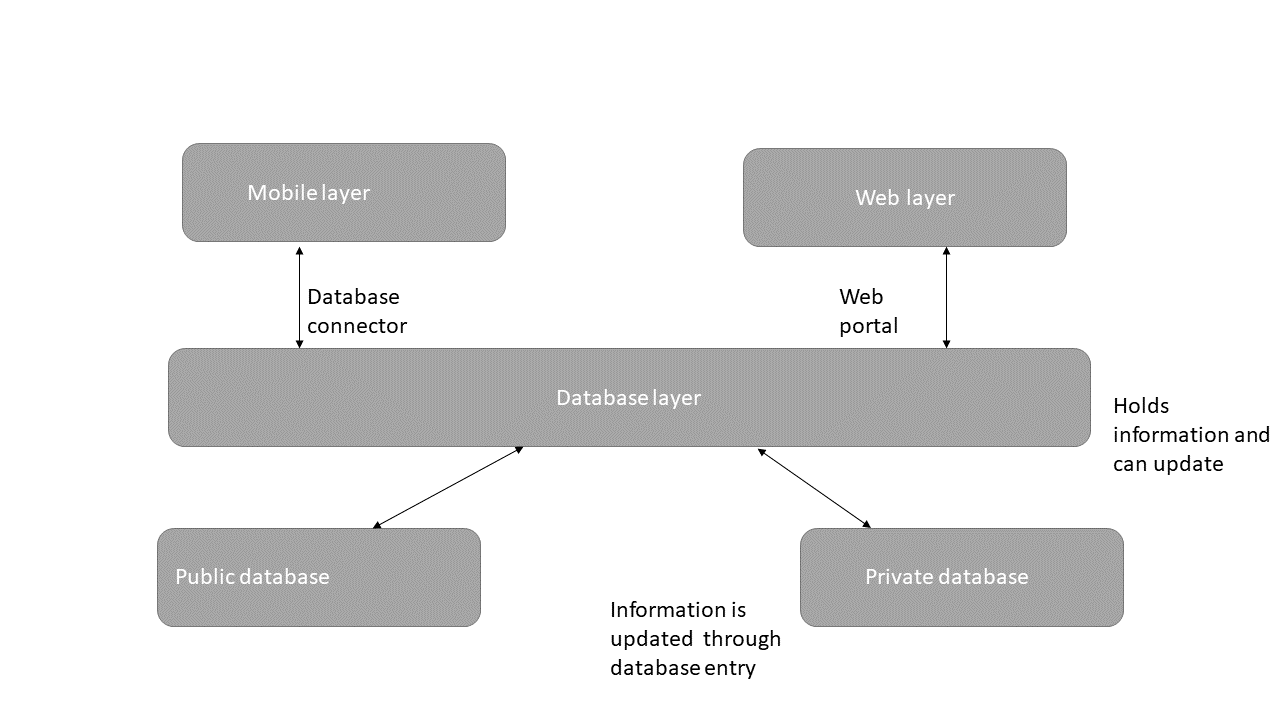
\includegraphics[width=0.60\textwidth]{images/database.pnj}
 \caption{Example subsystem description diagram}
\end{figure}

\subsubsection{Assumptions}

When the mobile layer or web layer requests the data or seems to change it from pubic database the database does the required task and displays inthe respected layer or it connects to private database to create or get infromation already created.

\subsubsection{Responsibilities}

When the mobile layer or web layer requests the data from public database the database does the required task and displays inthe respected layer
\subsubsection{Subsystem Interfaces}
It will be simitlar to public database used.
\begin {table}[H]
\caption {Subsystem interfaces} 
\begin{center}
    \begin{tabular}{ | p{1cm} | p{6cm} | p{3cm} | p{3cm} |}
    \hline
    ID & Description & Inputs & Outputs \\ \hline
   \#01 & Web portal and databse connector & \pbox{3cm}{local database } & \pbox{3cm}{expanded information \\ on brewery product}  \\ \hline
        \end{tabular}
\end{center}
\end{table}

\subsection{Subsystem 2}
This subsytem consist of the private database. So when the web application or mobile layer uses database connectors or the web portal to find the required information if the the inforamtion is not stored in the public database they go to this database which allows to create the required information or the already existinfg one is provided and displayed in the reqiured layer.

\subsubsection{Assumptions}
When the mobile layer or web layer requests the data and is not availbale from pubic database the database does it connects to private database to create or get requested infromation already created in private database.

\subsubsection{Responsibilities}

When the mobile layer or web layer requests the data or seems to change it from database layer the database does the required task and displays inthe respected layer


\subsubsection{Subsystem Interfaces}

\begin {table}[H]
\caption {Subsystem interfaces} 
\begin{center}
    \begin{tabular}{ | p{1cm} | p{6cm} | p{3cm} | p{3cm} |}
    \hline
    ID & Description & Inputs & Outputs \\ \hline
   \#01 & Web portal and databse connector & \pbox{3cm}{private database } & \pbox{3cm}{expanded information \\ on brewery product}  \\ \hline
        \end{tabular}
\end{center}
\end{table}
